% !TEX encoding = UTF-8 Unicode
% лекции 3-4, 20 февраля 2016
% вопросы 6-8
% 6. Задача Коши для одномерного волнового уравнения (колебания бесконечной струны). Вывод формулы Даламбера при помощи транспортного уравнения. Свойства решения. Волновые конусы. Конечная скорость распространения волн. Передний и задний фронт волны.
% 7-8. Канонический вид уравнений в частных производных

\subsection{Задача Коши для одномерного волнового уравнения}
Будем считать, что струна настолько длинная, что краевыми эффектами того, что струна зажата на концах, можно пренебречь. То есть, что струна просто колеблется в соответствии с нашим волновым уравнением. Волновое уравнение - один из тех редких случаев, когда можно получить общую формулу решения.
Решение выведем двумя способами.
\subsubsection{Вывод при помощи транспортного уравнения}
\begin{gather*}
	u_{tt} - v^2 u_{xx} = (\pder{t} - v \pder{x}) \underbrace {(\pder[u]{t} + v \pder[u]{x})}_{= w} = 0, \\
 	\pder[w]{t} - v \pder[w]{x} = 0.
\end{gather*}

Получили однородное транспортное уравнение, его решение мы знаем:
\begin{gather*}
	w(t,x) = \psi (x + vt),\quad \psi (x) = w(0,x) \\
	\pder[u]{t} + v \pder[u]{x} = \psi (x + vt)		
\end{gather*}

Получили неоднородное транспортное уравнение, его решение мы тоже знаем:
\begin{gather*}
	u(t,x) = u_0 (x - vt) + \int \limits_0^t \psi(x + vs - v(t-s)) ds = u_0 (x - vt) + \int \limits_0^t \psi (x - vt + 2vs) ds, \\
	\text{сделаем замену }y = x - vt + 2vs, \text{ тогда} \\
\end{gather*}
\begin{equation}
    u(t,x) = u_0 (x - vt) + \frac {1} {2v} \int \limits_{x-vt}^{x+vt} \psi (y) dy
\label{wavehomans}
\end{equation}

\begin{exercise}
При каких $\varphi$ и $\phi$ $\eqref{wavehomans}$ - решение $\eqref{waveequation}$? 
\end{exercise}
Ответ: $\varphi \in C^2$, $\psi \in C^1$.

Имем общее решение волнового уравнения. Поставим для него задачу Коши:

\begin{align}
    \begin{cases} 
        u_{tt} - v^2 u_{xx} = 0, \\
        u (0, x) = u_0 (x), \\
        u_t(0,x) = v_0 (x).
    \end{cases}
\label{wavecauchy}
\end{align}

\begin{theorem} Пусть $\varphi \in C^2(\real)$ и $\phi \in C^1(\real)$. Тогда
$$ u(t, x) = \varphi (x - vt) + \frac {1} {2v} \int \limits_{x - vt}^{x+vt} \psi (y) dy$$
--- решение задачи Коши для одномерного волнового уравнения $\ref{wavecauchy}$.
\end{theorem}
\begin{proof}
Подставляя $(0,x)$ в общее решение, получаем $$ u_0(x) = \varphi(x) .$$ Найдём $v_0(x)$:
\begin{gather*}
	u_t(0,x) = v_0(x) = \frac {1} {2v} (v \psi (x + vt) + v \psi (x - vt)) \Bigg\rvert_{t = 0} - v \varphi' (x)
	= \psi(x) - v \varphi'(x), \\
	\psi(x) = v_0(x) + v u'_0(x).
\end{gather*}
Таким образом,
\begin{align*}
	u(t,x) &= u_0(x-vt) + \frac {1} {2v} \int \limits_{x-vt}^{x+vt} v_0(y) + vu'_0(y)dy \\
	&= u_0(x-vt) + \frac {u_0(x+vt) - u_0(x-vt)} { 2} + \frac {1} {2v} \int \limits_{x-vt}^{x+vt} v_0(y)dy.
\end{align*}
Отсюда легко получаем формулу Д'Аламбера
\begin{equation}
	u(t,x) = \frac {u_0(x+vt) + u_0(x-vt)} { 2} + \frac {1} {2v} \int \limits_{x-vt}^{x+vt} v_0(y)dy.
\label{wavedalembert}
\end{equation}
\end{proof}

Сформулируем теорему:
\begin{theorem} Пусть $u_0 \in C^2(\real)$ и $v_0 \in C^1(\real)$, тогда формула Д'Аламбера $\eqref{wavedalembert}$ - единственное классическое решение задачи Коши для уравнения колебания бесконечной струны.
\end{theorem}

\begin{example}
Пусть $t$ - время, $x$ - координата вдоль струны. Предположим, на струне в точке $x_0$ сидит муравей. (Мировая линия объекта - траектория его движения в координатах пространства и времени) Пусть для простоты он не двигается. $x(t)$ - мировая линия, $v_0 = 0$. $x + vt = const$ и $x -vt = const$ - характеристические функции.

%TODO: рисунок про конусы
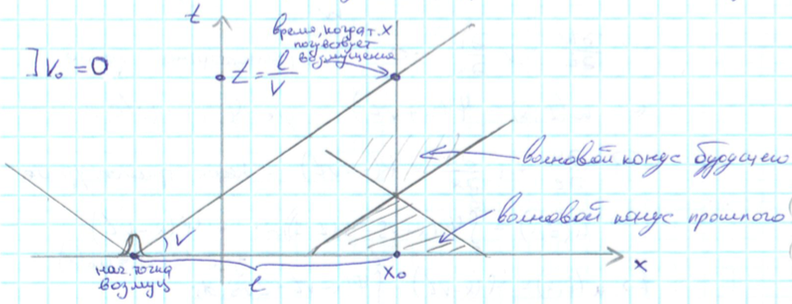
\includegraphics[scale=0.5]{part2.1.png}

Допустим, кто-то в точке [??] ударил по струне, для простоты пусть этот кто-то её отклонил, но не придал никакой начальной скорости ($v_0 = 0$, $u_0 \neq 0$). Когда муравей узнает о том, что что-то произошло? В момент времени $ t = \frac {l} {v}$, где $l$ - расстояние от муравья до источника возмущения, $v$ - скорость распространения возмущения. Будем считать, что профиль возмущения локализован около точки, тогда профиль распространяется вперёд и назад: бегут две волны. Если бы щелчок по струне был локализован в одной точке (тогда это не было бы классическим решением!), то муравей почуствовал бы фронт волны только на мгновение.
Интегрируем по содержимому конуса прошлого. Задав скорость муравью, можно повлиять на содержимое конуса будущего.
\end{example}

А что будет в трёхмерном случае? Распространение сферических волн. В отличие от формулы Д'Аламбера, не будет разницы между начальным возмущением с некоторой начальной скоростью и без неё. То есть, сферические фронты будут доходить от каждой точки волны. Сначала дойдёт передний фронт, потом задний.
А в двумерном? Распространение цилиндрических волн. Пример - берём удочку с поплавком, идём на пруд без течения. Забрасываем удочку, бросаем далеко от поплавка камушек. Получится примерно точечное возмущение. В какой-то момент передний фронт дойдёт до поплавка и он начнёт дёргаться. Волна пройдёт, а поплавок продолжит свои колебания, теоретически - бесконечно долго. То есть, заднего фронта не будет.

% Ч Т О ?
% TODO: написать что-нибудь нормальное

\subsubsection{Вывод решения при помощи замены переменных}
$$u_{tt} - v^2 u_{xx} = 0$$
Сделаем замену $(t, x) \to (\xi, \eta)$:
$$ \xi = x + vt, \quad \eta = x - vt.$$
\begin{align*}
	u_x &= u_{\xi} \xi_x + u_{\eta} \eta_x = u_{\xi} + u_{\eta}, \\
	u_t &=  u_{\xi} \xi_t + u_{\eta} \eta_t = v u_{\xi} + v u_{\eta}, \\
	u_{xx} &= u_{x\xi} \xi_x + u_{x\eta} \eta_x = u_{\xi\xi} + u_{\eta\xi} + u_{\xi\eta} + u_{\eta\eta}  =  u_{\xi\xi} + 2 u_{\xi\eta} + u_{\eta\eta}, \\
	u_{tt} &= u_{t\xi} \xi_t + u_{t\eta} \eta_t = v^2 (u_{\xi\xi} - u_{\eta\xi}) - v^2 (u_{\xi\eta} - u_{\eta\eta}) = v^2 (u_{\xi\xi} - 2u_{\xi\eta} + u_{\eta\eta}). \\
	\square_v u &= v^2 u_{\xi\xi} - 2v^2 u_{\xi\eta} + v^2 u_{\eta\eta} - v^2 u_{\xi\xi} - 2v^2 u_{\xi\eta} - v^2 u_{\eta\eta} = 0, \\
	u_{\xi\eta} &= 0, \quad u_{\xi} = F(\xi), \\
	u &= \int F(\xi) d\xi = \varphi (\xi) + \psi (\eta). \\
\end{align*}
Таким образом,
$$ u = \underbrace {\varphi (x+vt)}_{\text{волна направо}} + \underbrace {\psi (x-vt)}_{\text{волна налево}}.$$

Решим задачу Коши $\eqref{wavecauchy}$:
\begin{gather*}
	\begin{cases}
		u(0,x) = u_0(x) = \varphi(x) + \psi(x), \\
		u_t(0,x) = v_0(x) = v \varphi'(x) - v \psi(x),
	\end{cases}
	\begin{cases}
		\psi(x) = u_0(x) - \varphi(x), \\
		\varphi'(x)  - vu'_0(x) + v \varphi'(x) = v_0(x).
	\end{cases} \\
	\varphi'(x) = \frac {1} {2v} (v_0(x) + vu'_0(x)), \quad 	\varphi(x) = \frac {1} {2v} \int \limits_0^x v_0(y) + vu'_0(x) dy + C, \\
	\psi(x) = u_0 - \frac {1} {2v} \int \limits_0^x v_0(y) + vu'_0(y) dy - C,
\end{gather*}
Тогда
\begin{align*}
	u(t,x) &= \frac {1} {2v} \int \limits_0^{x+vt} v_0(y) + vu'_0(y) + C + u_0(x-vt) -  \frac {1} {2v} \int \limits_0^{x-vt} v_0(y) + vu'_0(y) dy - C \\
		&= u_0(x-vt) + \frac {1} {2v} \int \limits_{x-vt}^{x+vt} v_0(y) + v u'_0(y) dy.
\end{align*}
Отсюда легко получается та же самая формула Д'Аламбера \eqref{wavedalembert}:
\begin{equation*}
	u(t,x) = \frac {u_0(x+vt) + u_0(x-vt)} {2} + \frac {1} {2v} \int \limits_{x-vt}^{x+vt} v_0(y)dy.
\end{equation*}

% ЛЕНЬ
\subsection{Приведение уравнений второго порядка к каноническому виду в случае двух независимых переменных}
TODO
\subsection{Классификация уравнений второго порядка в случае многих независимых переменных}
TODO